\documentclass[twoside]{book}

% Packages required by doxygen
\usepackage{fixltx2e}
\usepackage{calc}
\usepackage{doxygen}
\usepackage[export]{adjustbox} % also loads graphicx
\usepackage{graphicx}
\usepackage[utf8]{inputenc}
\usepackage{makeidx}
\usepackage{multicol}
\usepackage{multirow}
\PassOptionsToPackage{warn}{textcomp}
\usepackage{textcomp}
\usepackage[nointegrals]{wasysym}
\usepackage[table]{xcolor}

% Font selection
\usepackage[T1]{fontenc}
\usepackage[scaled=.90]{helvet}
\usepackage{courier}
\usepackage{amssymb}
\usepackage{sectsty}
\renewcommand{\familydefault}{\sfdefault}
\allsectionsfont{%
  \fontseries{bc}\selectfont%
  \color{darkgray}%
}
\renewcommand{\DoxyLabelFont}{%
  \fontseries{bc}\selectfont%
  \color{darkgray}%
}
\newcommand{\+}{\discretionary{\mbox{\scriptsize$\hookleftarrow$}}{}{}}

% Page & text layout
\usepackage{geometry}
\geometry{%
  a4paper,%
  top=2.5cm,%
  bottom=2.5cm,%
  left=2.5cm,%
  right=2.5cm%
}
\tolerance=750
\hfuzz=15pt
\hbadness=750
\setlength{\emergencystretch}{15pt}
\setlength{\parindent}{0cm}
\setlength{\parskip}{3ex plus 2ex minus 2ex}
\makeatletter
\renewcommand{\paragraph}{%
  \@startsection{paragraph}{4}{0ex}{-1.0ex}{1.0ex}{%
    \normalfont\normalsize\bfseries\SS@parafont%
  }%
}
\renewcommand{\subparagraph}{%
  \@startsection{subparagraph}{5}{0ex}{-1.0ex}{1.0ex}{%
    \normalfont\normalsize\bfseries\SS@subparafont%
  }%
}
\makeatother

% Headers & footers
\usepackage{fancyhdr}
\pagestyle{fancyplain}
\fancyhead[LE]{\fancyplain{}{\bfseries\thepage}}
\fancyhead[CE]{\fancyplain{}{}}
\fancyhead[RE]{\fancyplain{}{\bfseries\leftmark}}
\fancyhead[LO]{\fancyplain{}{\bfseries\rightmark}}
\fancyhead[CO]{\fancyplain{}{}}
\fancyhead[RO]{\fancyplain{}{\bfseries\thepage}}
\fancyfoot[LE]{\fancyplain{}{}}
\fancyfoot[CE]{\fancyplain{}{}}
\fancyfoot[RE]{\fancyplain{}{\bfseries\scriptsize Generated by Doxygen }}
\fancyfoot[LO]{\fancyplain{}{\bfseries\scriptsize Generated by Doxygen }}
\fancyfoot[CO]{\fancyplain{}{}}
\fancyfoot[RO]{\fancyplain{}{}}
\renewcommand{\footrulewidth}{0.4pt}
\renewcommand{\chaptermark}[1]{%
  \markboth{#1}{}%
}
\renewcommand{\sectionmark}[1]{%
  \markright{\thesection\ #1}%
}

% Indices & bibliography
\usepackage{natbib}
\usepackage[titles]{tocloft}
\setcounter{tocdepth}{3}
\setcounter{secnumdepth}{5}
\makeindex

% Hyperlinks (required, but should be loaded last)
\usepackage{ifpdf}
\ifpdf
  \usepackage[pdftex,pagebackref=true]{hyperref}
\else
  \usepackage[ps2pdf,pagebackref=true]{hyperref}
\fi
\hypersetup{%
  colorlinks=true,%
  linkcolor=blue,%
  citecolor=blue,%
  unicode%
}

% Custom commands
\newcommand{\clearemptydoublepage}{%
  \newpage{\pagestyle{empty}\cleardoublepage}%
}

\usepackage{caption}
\captionsetup{labelsep=space,justification=centering,font={bf},singlelinecheck=off,skip=4pt,position=top}

%===== C O N T E N T S =====

\begin{document}

% Titlepage & ToC
\hypersetup{pageanchor=false,
             bookmarksnumbered=true,
             pdfencoding=unicode
            }
\pagenumbering{roman}
\begin{titlepage}
\vspace*{7cm}
\begin{center}%
{\Large C\+M\+P\+E352 Project }\\
\vspace*{1cm}
{\large Generated by Doxygen 1.8.11}\\
\end{center}
\end{titlepage}
\clearemptydoublepage
\tableofcontents
\clearemptydoublepage
\pagenumbering{arabic}
\hypersetup{pageanchor=true}

%--- Begin generated contents ---
\chapter{Hierarchical Index}
\section{Class Hierarchy}
This inheritance list is sorted roughly, but not completely, alphabetically\+:\begin{DoxyCompactList}
\item \contentsline{section}{com.\+mert.\+Genre}{\pageref{classcom_1_1mert_1_1_genre}}{}
\item \contentsline{section}{com.\+mert.\+test.\+Genre\+Test}{\pageref{classcom_1_1mert_1_1test_1_1_genre_test}}{}
\item \contentsline{section}{com.\+mert.\+test.\+Main\+Servlet\+Test}{\pageref{classcom_1_1mert_1_1test_1_1_main_servlet_test}}{}
\item \contentsline{section}{com.\+mert.\+test.\+Update\+D\+B\+Test}{\pageref{classcom_1_1mert_1_1test_1_1_update_d_b_test}}{}
\item Http\+Servlet\begin{DoxyCompactList}
\item \contentsline{section}{com.\+mert.\+Main\+Servlet}{\pageref{classcom_1_1mert_1_1_main_servlet}}{}
\item \contentsline{section}{com.\+mert.\+Save\+Entries}{\pageref{classcom_1_1mert_1_1_save_entries}}{}
\item \contentsline{section}{com.\+mert.\+Search}{\pageref{classcom_1_1mert_1_1_search}}{}
\item \contentsline{section}{com.\+mert.\+Show\+Entries}{\pageref{classcom_1_1mert_1_1_show_entries}}{}
\item \contentsline{section}{com.\+mert.\+Show\+Movies}{\pageref{classcom_1_1mert_1_1_show_movies}}{}
\item \contentsline{section}{com.\+mert.\+Update\+DB}{\pageref{classcom_1_1mert_1_1_update_d_b}}{}
\end{DoxyCompactList}
\end{DoxyCompactList}

\chapter{Class Index}
\section{Class List}
Here are the classes, structs, unions and interfaces with brief descriptions\+:\begin{DoxyCompactList}
\item\contentsline{section}{\hyperlink{classplanets_1_1_main_servlet}{planets.\+Main\+Servlet} }{\pageref{classplanets_1_1_main_servlet}}{}
\end{DoxyCompactList}

\chapter{File Index}
\section{File List}
Here is a list of all files with brief descriptions\+:\begin{DoxyCompactList}
\item\contentsline{section}{C\+:/\+Users/\+Kaan\+Bulut/workspace/\+Test\+Cities/src/\hyperlink{_city_search_8java}{City\+Search.\+java} }{\pageref{_city_search_8java}}{}
\item\contentsline{section}{C\+:/\+Users/\+Kaan\+Bulut/workspace/\+Test\+Cities/src/\hyperlink{_city_search_test_8java}{City\+Search\+Test.\+java} }{\pageref{_city_search_test_8java}}{}
\end{DoxyCompactList}

\chapter{Class Documentation}
\hypertarget{class_city_search}{}\section{City\+Search Class Reference}
\label{class_city_search}\index{City\+Search@{City\+Search}}


Servlet for a website on city search.  


Inheritance diagram for City\+Search\+:\begin{figure}[H]
\begin{center}
\leavevmode
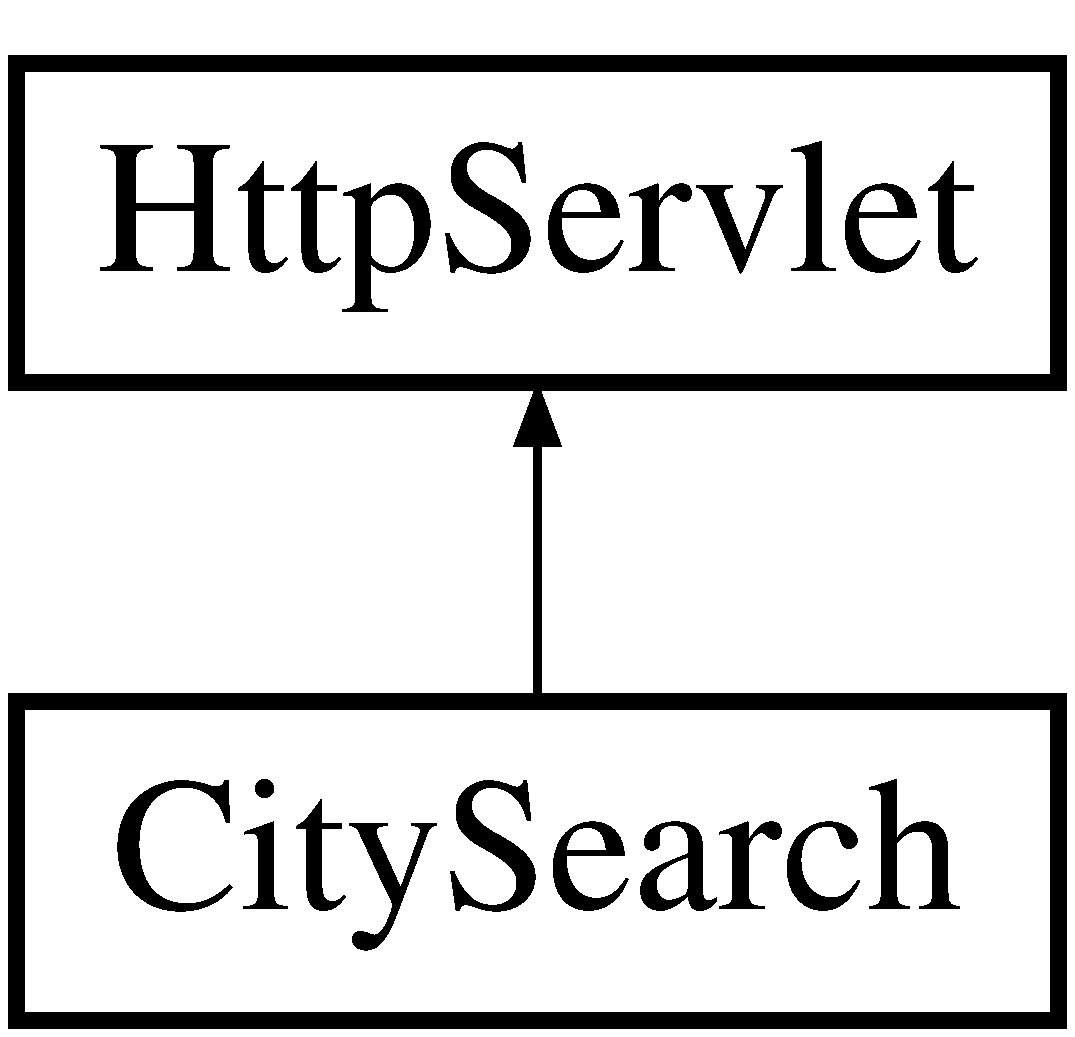
\includegraphics[height=2.000000cm]{class_city_search}
\end{center}
\end{figure}
\subsection*{Public Member Functions}
\begin{DoxyCompactItemize}
\item 
Array\+List$<$ Hash\+Map$<$ String, String $>$ $>$ \hyperlink{class_city_search_aa89f03a8e1e1ba6b4cca39d3a77d0aea}{run\+Query} (String query)
\item 
String \hyperlink{class_city_search_ad3169a9a050fb3efcc480eb9d4a31601}{get\+Query\+Body} (Http\+Servlet\+Request request)
\item 
Array\+List$<$ Hash\+Map$<$ String, String $>$ $>$ \hyperlink{class_city_search_a79b7b631af176e21aac968101fe4eb0d}{run\+Data\+Query} (Http\+Servlet\+Request request)
\item 
String \hyperlink{class_city_search_ae95f20000b6ffd73f58e20841a344c33}{get\+Options} (Http\+Servlet\+Request request)
\item 
String \hyperlink{class_city_search_a52cde722fb752e78e377a879d776041d}{get\+Table} (Http\+Servlet\+Request request)
\item 
String \hyperlink{class_city_search_a7ebefad5e5a6c895cf2f8bc350779165}{get\+Page\+Menu} (Http\+Servlet\+Request request)
\item 
String \hyperlink{class_city_search_ad8fa69bece192ae293c2dd96e614e337}{generate\+H\+T\+ML} (Http\+Servlet\+Request request)
\item 
void \hyperlink{class_city_search_ab392666fdc0948b40d90af4715429451}{init} ()  throws Servlet\+Exception 
\item 
void \hyperlink{class_city_search_a9e1fc3bb51d58588be7d55c80d97bc82}{do\+Get} (Http\+Servlet\+Request request, Http\+Servlet\+Response response)  throws Servlet\+Exception, I\+O\+Exception 
\item 
void \hyperlink{class_city_search_a1b194c808d33eb362a07eb4a87a6995f}{do\+Post} (Http\+Servlet\+Request request, Http\+Servlet\+Response response)  throws Servlet\+Exception, I\+O\+Exception 
\item 
void \hyperlink{class_city_search_a4fcacbf97c43741eff5acf8dd091f495}{destroy} ()
\end{DoxyCompactItemize}


\subsection{Detailed Description}
Servlet for a website on city search. 

This servlet creates a webpage where you can search cities by name, country and population. It also allows results to be saved to a database.

\begin{DoxyVersion}{Version}
1.\+0 
\end{DoxyVersion}
\begin{DoxyAuthor}{Author}
Kaan Bulut Tekelioglu 
\end{DoxyAuthor}
\begin{DoxyDate}{Date}
May 2016 
\end{DoxyDate}


\subsection{Member Function Documentation}
\index{City\+Search@{City\+Search}!destroy@{destroy}}
\index{destroy@{destroy}!City\+Search@{City\+Search}}
\subsubsection[{\texorpdfstring{destroy()}{destroy()}}]{\setlength{\rightskip}{0pt plus 5cm}void City\+Search.\+destroy (
\begin{DoxyParamCaption}
{}
\end{DoxyParamCaption}
)}\hypertarget{class_city_search_a4fcacbf97c43741eff5acf8dd091f495}{}\label{class_city_search_a4fcacbf97c43741eff5acf8dd091f495}
Disconnects from the database when the servlet is destroyed. \index{City\+Search@{City\+Search}!do\+Get@{do\+Get}}
\index{do\+Get@{do\+Get}!City\+Search@{City\+Search}}
\subsubsection[{\texorpdfstring{do\+Get(\+Http\+Servlet\+Request request, Http\+Servlet\+Response response)}{doGet(HttpServletRequest request, HttpServletResponse response)}}]{\setlength{\rightskip}{0pt plus 5cm}void City\+Search.\+do\+Get (
\begin{DoxyParamCaption}
\item[{Http\+Servlet\+Request}]{request, }
\item[{Http\+Servlet\+Response}]{response}
\end{DoxyParamCaption}
) throws Servlet\+Exception, I\+O\+Exception}\hypertarget{class_city_search_a9e1fc3bb51d58588be7d55c80d97bc82}{}\label{class_city_search_a9e1fc3bb51d58588be7d55c80d97bc82}
Prints the H\+T\+ML code when a G\+ET request is made.


\begin{DoxyParams}{Parameters}
{\em request} & 
\begin{DoxyItemize}
\item The H\+T\+TP request. 
\end{DoxyItemize}\\
\hline
{\em response} & 
\begin{DoxyItemize}
\item The H\+T\+TP response of this servlet. 
\end{DoxyItemize}\\
\hline
\end{DoxyParams}
\index{City\+Search@{City\+Search}!do\+Post@{do\+Post}}
\index{do\+Post@{do\+Post}!City\+Search@{City\+Search}}
\subsubsection[{\texorpdfstring{do\+Post(\+Http\+Servlet\+Request request, Http\+Servlet\+Response response)}{doPost(HttpServletRequest request, HttpServletResponse response)}}]{\setlength{\rightskip}{0pt plus 5cm}void City\+Search.\+do\+Post (
\begin{DoxyParamCaption}
\item[{Http\+Servlet\+Request}]{request, }
\item[{Http\+Servlet\+Response}]{response}
\end{DoxyParamCaption}
) throws Servlet\+Exception, I\+O\+Exception}\hypertarget{class_city_search_a1b194c808d33eb362a07eb4a87a6995f}{}\label{class_city_search_a1b194c808d33eb362a07eb4a87a6995f}
Writes U\+R\+Ls to database when a P\+O\+ST request is made.


\begin{DoxyParams}{Parameters}
{\em request} & 
\begin{DoxyItemize}
\item The H\+T\+TP request. 
\end{DoxyItemize}\\
\hline
{\em response} & 
\begin{DoxyItemize}
\item The H\+T\+TP response of this servlet. 
\end{DoxyItemize}\\
\hline
\end{DoxyParams}
\index{City\+Search@{City\+Search}!generate\+H\+T\+ML@{generate\+H\+T\+ML}}
\index{generate\+H\+T\+ML@{generate\+H\+T\+ML}!City\+Search@{City\+Search}}
\subsubsection[{\texorpdfstring{generate\+H\+T\+M\+L(\+Http\+Servlet\+Request request)}{generateHTML(HttpServletRequest request)}}]{\setlength{\rightskip}{0pt plus 5cm}String City\+Search.\+generate\+H\+T\+ML (
\begin{DoxyParamCaption}
\item[{Http\+Servlet\+Request}]{request}
\end{DoxyParamCaption}
)}\hypertarget{class_city_search_ad8fa69bece192ae293c2dd96e614e337}{}\label{class_city_search_ad8fa69bece192ae293c2dd96e614e337}
Generates the H\+T\+ML code for the entire page.


\begin{DoxyParams}{Parameters}
{\em request} & 
\begin{DoxyItemize}
\item The H\+T\+TP request. 
\end{DoxyItemize}\\
\hline
\end{DoxyParams}
\begin{DoxyReturn}{Returns}
The H\+T\+ML code the entire page. 
\end{DoxyReturn}
\index{City\+Search@{City\+Search}!get\+Options@{get\+Options}}
\index{get\+Options@{get\+Options}!City\+Search@{City\+Search}}
\subsubsection[{\texorpdfstring{get\+Options(\+Http\+Servlet\+Request request)}{getOptions(HttpServletRequest request)}}]{\setlength{\rightskip}{0pt plus 5cm}String City\+Search.\+get\+Options (
\begin{DoxyParamCaption}
\item[{Http\+Servlet\+Request}]{request}
\end{DoxyParamCaption}
)}\hypertarget{class_city_search_ae95f20000b6ffd73f58e20841a344c33}{}\label{class_city_search_ae95f20000b6ffd73f58e20841a344c33}
Creates the H\+T\+ML code for a dropdown menu for sort selection.


\begin{DoxyParams}{Parameters}
{\em request} & 
\begin{DoxyItemize}
\item The H\+T\+TP request. 
\end{DoxyItemize}\\
\hline
\end{DoxyParams}
\begin{DoxyReturn}{Returns}
The H\+T\+ML code for the dropdown menu. 
\end{DoxyReturn}
\index{City\+Search@{City\+Search}!get\+Page\+Menu@{get\+Page\+Menu}}
\index{get\+Page\+Menu@{get\+Page\+Menu}!City\+Search@{City\+Search}}
\subsubsection[{\texorpdfstring{get\+Page\+Menu(\+Http\+Servlet\+Request request)}{getPageMenu(HttpServletRequest request)}}]{\setlength{\rightskip}{0pt plus 5cm}String City\+Search.\+get\+Page\+Menu (
\begin{DoxyParamCaption}
\item[{Http\+Servlet\+Request}]{request}
\end{DoxyParamCaption}
)}\hypertarget{class_city_search_a7ebefad5e5a6c895cf2f8bc350779165}{}\label{class_city_search_a7ebefad5e5a6c895cf2f8bc350779165}
Creates the H\+T\+ML code for a table to select pages of the query result.


\begin{DoxyParams}{Parameters}
{\em request} & 
\begin{DoxyItemize}
\item The H\+T\+TP request. 
\end{DoxyItemize}\\
\hline
\end{DoxyParams}
\begin{DoxyReturn}{Returns}
The H\+T\+ML code for a table to select pages. 
\end{DoxyReturn}
\index{City\+Search@{City\+Search}!get\+Query\+Body@{get\+Query\+Body}}
\index{get\+Query\+Body@{get\+Query\+Body}!City\+Search@{City\+Search}}
\subsubsection[{\texorpdfstring{get\+Query\+Body(\+Http\+Servlet\+Request request)}{getQueryBody(HttpServletRequest request)}}]{\setlength{\rightskip}{0pt plus 5cm}String City\+Search.\+get\+Query\+Body (
\begin{DoxyParamCaption}
\item[{Http\+Servlet\+Request}]{request}
\end{DoxyParamCaption}
)}\hypertarget{class_city_search_ad3169a9a050fb3efcc480eb9d4a31601}{}\label{class_city_search_ad3169a9a050fb3efcc480eb9d4a31601}
Runs the body of the data extraction query for city search. It does filtering in the query according to parameters in request.


\begin{DoxyParams}{Parameters}
{\em request} & 
\begin{DoxyItemize}
\item The H\+T\+TP request. 
\end{DoxyItemize}\\
\hline
\end{DoxyParams}
\begin{DoxyReturn}{Returns}
The body of the query. 
\end{DoxyReturn}
\index{City\+Search@{City\+Search}!get\+Table@{get\+Table}}
\index{get\+Table@{get\+Table}!City\+Search@{City\+Search}}
\subsubsection[{\texorpdfstring{get\+Table(\+Http\+Servlet\+Request request)}{getTable(HttpServletRequest request)}}]{\setlength{\rightskip}{0pt plus 5cm}String City\+Search.\+get\+Table (
\begin{DoxyParamCaption}
\item[{Http\+Servlet\+Request}]{request}
\end{DoxyParamCaption}
)}\hypertarget{class_city_search_a52cde722fb752e78e377a879d776041d}{}\label{class_city_search_a52cde722fb752e78e377a879d776041d}
Creates the H\+T\+ML code for the results table.


\begin{DoxyParams}{Parameters}
{\em request} & 
\begin{DoxyItemize}
\item The H\+T\+TP request. 
\end{DoxyItemize}\\
\hline
\end{DoxyParams}
\begin{DoxyReturn}{Returns}
The H\+T\+ML code for the results table. 
\end{DoxyReturn}
\index{City\+Search@{City\+Search}!init@{init}}
\index{init@{init}!City\+Search@{City\+Search}}
\subsubsection[{\texorpdfstring{init()}{init()}}]{\setlength{\rightskip}{0pt plus 5cm}void City\+Search.\+init (
\begin{DoxyParamCaption}
{}
\end{DoxyParamCaption}
) throws Servlet\+Exception}\hypertarget{class_city_search_ab392666fdc0948b40d90af4715429451}{}\label{class_city_search_ab392666fdc0948b40d90af4715429451}
Initializes the database connection. \index{City\+Search@{City\+Search}!run\+Data\+Query@{run\+Data\+Query}}
\index{run\+Data\+Query@{run\+Data\+Query}!City\+Search@{City\+Search}}
\subsubsection[{\texorpdfstring{run\+Data\+Query(\+Http\+Servlet\+Request request)}{runDataQuery(HttpServletRequest request)}}]{\setlength{\rightskip}{0pt plus 5cm}Array\+List$<$Hash\+Map$<$String, String$>$ $>$ City\+Search.\+run\+Data\+Query (
\begin{DoxyParamCaption}
\item[{Http\+Servlet\+Request}]{request}
\end{DoxyParamCaption}
)}\hypertarget{class_city_search_a79b7b631af176e21aac968101fe4eb0d}{}\label{class_city_search_a79b7b631af176e21aac968101fe4eb0d}
Runs the query for data extraction. It sorts and pages data according to parameters.


\begin{DoxyParams}{Parameters}
{\em request} & 
\begin{DoxyItemize}
\item The H\+T\+TP request. 
\end{DoxyItemize}\\
\hline
\end{DoxyParams}
\begin{DoxyReturn}{Returns}
The result list for the data query. 
\end{DoxyReturn}
\index{City\+Search@{City\+Search}!run\+Query@{run\+Query}}
\index{run\+Query@{run\+Query}!City\+Search@{City\+Search}}
\subsubsection[{\texorpdfstring{run\+Query(\+String query)}{runQuery(String query)}}]{\setlength{\rightskip}{0pt plus 5cm}Array\+List$<$Hash\+Map$<$String, String$>$ $>$ City\+Search.\+run\+Query (
\begin{DoxyParamCaption}
\item[{String}]{query}
\end{DoxyParamCaption}
)}\hypertarget{class_city_search_aa89f03a8e1e1ba6b4cca39d3a77d0aea}{}\label{class_city_search_aa89f03a8e1e1ba6b4cca39d3a77d0aea}
Runs a given query in wikidata. The query must be valid. Returns an Array\+List of Hashmaps, where each row is a result, and column names are keys to the maps.


\begin{DoxyParams}{Parameters}
{\em query} & 
\begin{DoxyItemize}
\item The query to be run. 
\end{DoxyItemize}\\
\hline
\end{DoxyParams}
\begin{DoxyReturn}{Returns}
The result list. 
\end{DoxyReturn}


The documentation for this class was generated from the following file\+:\begin{DoxyCompactItemize}
\item 
C\+:/\+Users/\+Kaan\+Bulut/workspace/\+Test\+Cities/src/\hyperlink{_city_search_8java}{City\+Search.\+java}\end{DoxyCompactItemize}

\hypertarget{class_city_search_test}{}\section{City\+Search\+Test Class Reference}
\label{class_city_search_test}\index{City\+Search\+Test@{City\+Search\+Test}}
\subsection*{Public Member Functions}
\begin{DoxyCompactItemize}
\item 
void \hyperlink{class_city_search_test_a40943d78c1aaf777bed011e3ec424e70}{run\+Test\+Query} ()
\item 
void \hyperlink{class_city_search_test_ac77ed2f644a331be59bc803c70ce686c}{run\+Empty\+Query} ()
\end{DoxyCompactItemize}


\subsection{Detailed Description}
Unit tests for \hyperlink{class_city_search}{City\+Search}. \begin{DoxyAuthor}{Author}
Kaan\+Bulut 
\end{DoxyAuthor}


\subsection{Member Function Documentation}
\index{City\+Search\+Test@{City\+Search\+Test}!run\+Empty\+Query@{run\+Empty\+Query}}
\index{run\+Empty\+Query@{run\+Empty\+Query}!City\+Search\+Test@{City\+Search\+Test}}
\subsubsection[{\texorpdfstring{run\+Empty\+Query()}{runEmptyQuery()}}]{\setlength{\rightskip}{0pt plus 5cm}void City\+Search\+Test.\+run\+Empty\+Query (
\begin{DoxyParamCaption}
{}
\end{DoxyParamCaption}
)}\hypertarget{class_city_search_test_ac77ed2f644a331be59bc803c70ce686c}{}\label{class_city_search_test_ac77ed2f644a331be59bc803c70ce686c}
Tests for an empty query. \index{City\+Search\+Test@{City\+Search\+Test}!run\+Test\+Query@{run\+Test\+Query}}
\index{run\+Test\+Query@{run\+Test\+Query}!City\+Search\+Test@{City\+Search\+Test}}
\subsubsection[{\texorpdfstring{run\+Test\+Query()}{runTestQuery()}}]{\setlength{\rightskip}{0pt plus 5cm}void City\+Search\+Test.\+run\+Test\+Query (
\begin{DoxyParamCaption}
{}
\end{DoxyParamCaption}
)}\hypertarget{class_city_search_test_a40943d78c1aaf777bed011e3ec424e70}{}\label{class_city_search_test_a40943d78c1aaf777bed011e3ec424e70}
Tests for a query for the city Istanbul. 

The documentation for this class was generated from the following file\+:\begin{DoxyCompactItemize}
\item 
C\+:/\+Users/\+Kaan\+Bulut/workspace/\+Test\+Cities/src/\hyperlink{_city_search_test_8java}{City\+Search\+Test.\+java}\end{DoxyCompactItemize}

\chapter{File Documentation}
\hypertarget{_city_search_8java}{}\section{C\+:/\+Users/\+Kaan\+Bulut/workspace/\+Test\+Cities/src/\+City\+Search.java File Reference}
\label{_city_search_8java}\index{C\+:/\+Users/\+Kaan\+Bulut/workspace/\+Test\+Cities/src/\+City\+Search.\+java@{C\+:/\+Users/\+Kaan\+Bulut/workspace/\+Test\+Cities/src/\+City\+Search.\+java}}
\subsection*{Classes}
\begin{DoxyCompactItemize}
\item 
class \hyperlink{class_city_search}{City\+Search}
\begin{DoxyCompactList}\small\item\em Servlet for a website on city search. \end{DoxyCompactList}\end{DoxyCompactItemize}

\hypertarget{_city_search_test_8java}{}\section{C\+:/\+Users/\+Kaan\+Bulut/workspace/\+Test\+Cities/src/\+City\+Search\+Test.java File Reference}
\label{_city_search_test_8java}\index{C\+:/\+Users/\+Kaan\+Bulut/workspace/\+Test\+Cities/src/\+City\+Search\+Test.\+java@{C\+:/\+Users/\+Kaan\+Bulut/workspace/\+Test\+Cities/src/\+City\+Search\+Test.\+java}}
\subsection*{Classes}
\begin{DoxyCompactItemize}
\item 
class \hyperlink{class_city_search_test}{City\+Search\+Test}
\end{DoxyCompactItemize}

%--- End generated contents ---

% Index
\backmatter
\newpage
\phantomsection
\clearemptydoublepage
\addcontentsline{toc}{chapter}{Index}
\printindex

\end{document}
